\documentclass[conference]{IEEEtran}

\usepackage[utf8]{inputenc}
\usepackage{graphicx}
\usepackage{amsmath}
\usepackage{hyperref}
\usepackage[spanish]{babel}

\title{\LARGE\textbf{\textit{Prototipo de Simulador de Laboratorio de Química Inorgánica en Realidad Virtual}}}

\author{
    \IEEEauthorblockN{\large Marcos Martí Sandino Mictlantecuhtli García Aguayo,\\ Saul De La O Torres, Gabriel Sepúlveda Cervante}
    \IEEEauthorblockA{\normalsize Escuela Superior de Cómputo I.P.N. México CDMX\\
    Tel. 57-29-6000 ext 52000 y 52021. E-mail: \href{mailto:mgarciaa1711@alumno.ipn.mx}{mgarciaa1711@alumno.ipn.mx}}
}

\begin{document}

\maketitle

\begin{abstract}
Este trabajo presenta el desarrollo de un prototipo de simulador de laboratorio de química inorgánica en realidad virtual, orientado a la enseñanza inmersiva mediante tecnologías avanzadas como seguimiento de manos, sistemas FSM y una tabla periódica interactiva. El sistema permite realizar experimentos estructurados que abarcan balanceo de ecuaciones, creación de compuestos y simulación de reacciones químicas, integrando efectos visuales y auditivos en tiempo real. Validado por expertos.
\end{abstract}
\renewcommand\IEEEkeywordsname{Palabras clave}
\begin{IEEEkeywords}
Química Inorgánica, Realidad Virtual, Simulador, Software Interactivo.
\end{IEEEkeywords}

\section{Introducción}

En las últimas décadas, el avance tecnológico ha transformado diversos ámbitos de la sociedad, incluyendo el educativo, donde la integración de tecnologías innovadoras ha demostrado ser un factor clave para enfrentar los desafíos del aprendizaje. Según Brito \cite{Brito2015}, la cultura digital ha redefinido la producción, circulación y apropiación del conocimiento, desafiando las estructuras tradicionales y fomentando nuevos enfoques pedagógicos.

En México, a pesar de la implementación de programas destinados a incorporar herramientas tecnológicas en la educación básica, los resultados han sido limitados debido a la rigidez de las instituciones escolares y la falta de un replanteamiento en los modelos de enseñanza \cite{TrejoQuintana2020}. Sin embargo, la llegada de tecnologías como la realidad virtual (RV) abre nuevas posibilidades en el ámbito educativo, proporcionando experiencias inmersivas que permiten simular situaciones y entornos complejos, transformándose en herramientas valiosas para la enseñanza de disciplinas científicas como la química inorgánica \cite{Zapatero2011}.

La química inorgánica, una rama fundamental de la química, enfrenta retos importantes en su enseñanza debido a la abstracción de sus conceptos y la falta de recursos en los laboratorios. Esto resulta en un desinterés significativo entre los estudiantes hacia esta materia, obstaculizando el aprendizaje profundo de sus principios fundamentales. Ante esta problemática, se plantea el desarrollo de un prototipo de simulador de laboratorio de química inorgánica en RV como una solución innovadora para enriquecer la experiencia educativa.

Este simulador está diseñado para proporcionar un entorno controlado y seguro donde los estudiantes puedan interactuar con elementos químicos, observar reacciones en tiempo real y realizar actividades prácticas, como balanceo de ecuaciones y creación de compuestos. Su implementación busca no solo complementar el aprendizaje teórico, sino también fomentar un mayor interés en la química, incentivando una comprensión práctica y dinámica de los conceptos.

El proyecto responde a la necesidad de revitalizar la enseñanza de la química inorgánica mediante el uso de herramientas tecnológicas avanzadas. Al ofrecer una experiencia educativa interactiva y cautivadora, se pretende abordar la falta de interés de los estudiantes y promover su motivación intrínseca hacia las ciencias. Este enfoque, alineado con los principios de la educación STEM \cite{Zamorano2018}, se presenta como una solución viable para transformar el aprendizaje de la química en un proceso más atractivo y significativo.

En este documento se describen los antecedentes, la metodología, el desarrollo y los resultados de la validación del prototipo, con el objetivo de destacar su impacto potencial en la enseñanza de la química inorgánica y su contribución al ámbito educativo.

\section{Metodología}

El simulador de laboratorio de química inorgánica en realidad virtual está compuesto por módulos interconectados que gestionan de manera sincronizada las diversas funcionalidades del sistema. Cada módulo desempeña un rol específico dentro del flujo general del simulador, el cual incluye un tutorial introductorio y cuatro experimentos organizados en fases estructuradas. Este diseño modular asegura una experiencia educativa inmersiva y precisa.

\begin{figure}[thbp]
    \centering
    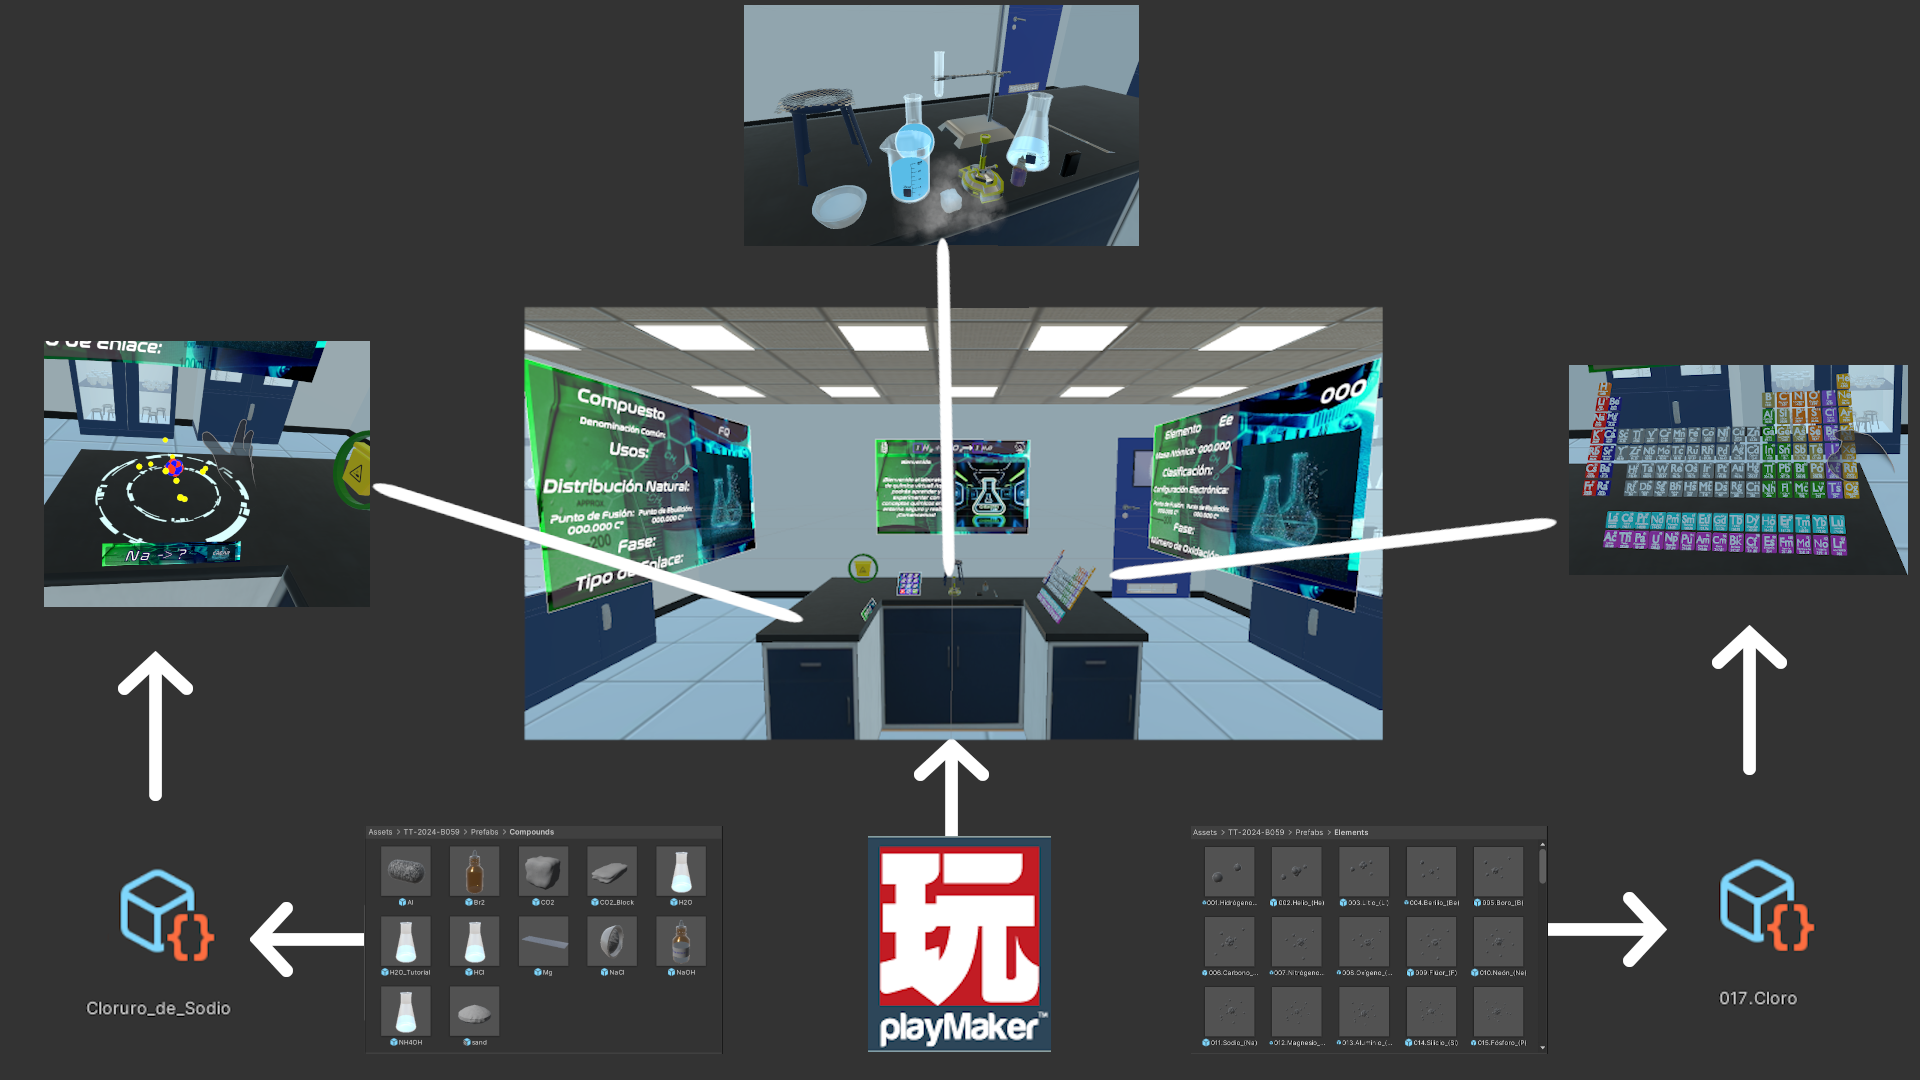
\includegraphics[width=0.45\textwidth, height = 5cm]{img/Lab2.png}
    \caption{Estructura General del Laboratorio}
    \label{fig:Estructura General del Laboratorio}
\end{figure}

\subsection{Flujo General del Simulador}

El simulador sigue una estructura base compuesta por las siguientes fases:
\begin{enumerate}
    \item \textbf{Introducción:} Presenta al usuario los objetivos y las herramientas del laboratorio virtual.
    \item \textbf{Balanceo de Ecuaciones:} Actividad guiada para reforzar los principios fundamentales de conservación de la materia.
    \item \textbf{Selección y Creación:} Interacción con la tabla periódica para seleccionar elementos y combinarlos.
    \item \textbf{Experimentación:} Realización práctica del experimento mediante el uso de instrumental virtual y compuestos.
    \item \textbf{Explicación:} Retroalimentación textual y visual sobre los resultados obtenidos.
\end{enumerate}

Cada fase está diseñada para facilitar un aprendizaje progresivo e interactivo, con transiciones gestionadas mediante máquinas de estados finitos (\textit{Finite State Machines}, FSM) integradas en los módulos principales.

\begin{figure}[thbp]
    \centering
    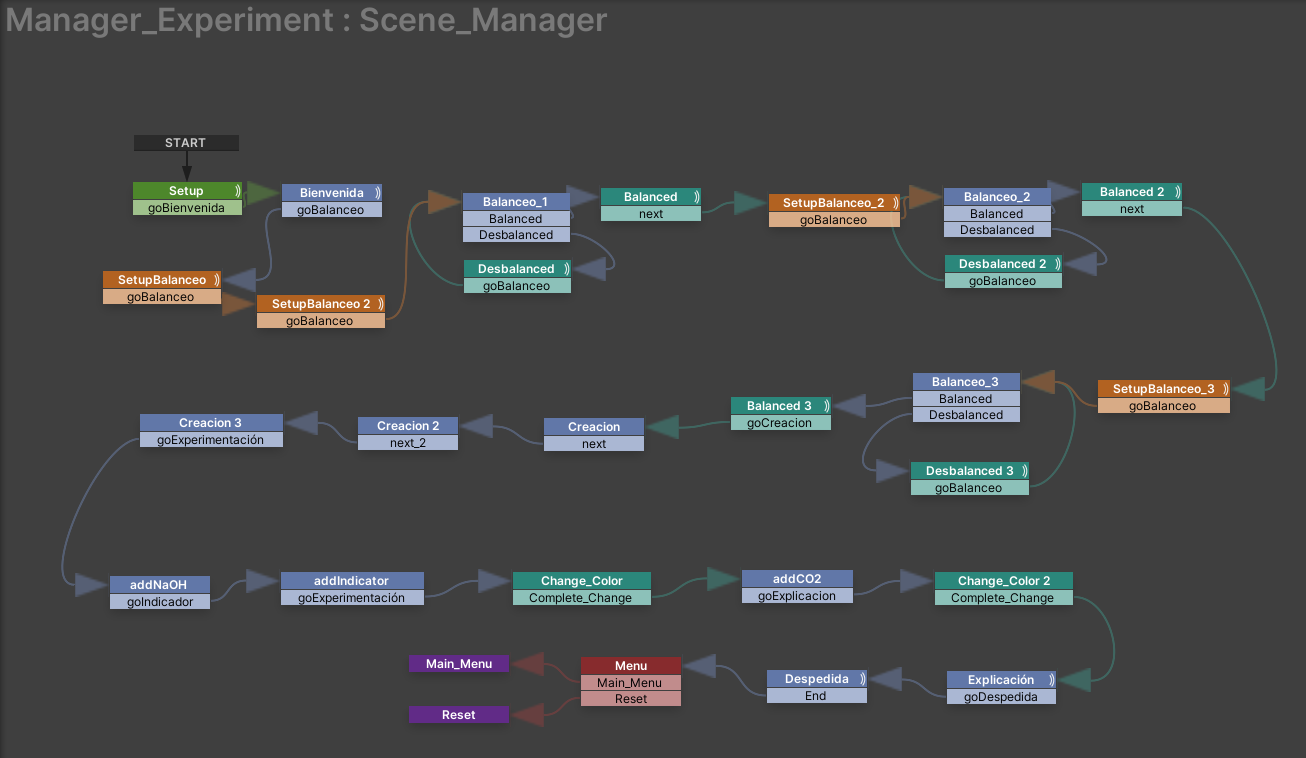
\includegraphics[width=0.45\textwidth, height = 5cm]{img/Experimento_01.png}
    \caption{Flujo General del Experimento}
    \label{fig:Flujo General del Experimento}
\end{figure}

\subsection{Módulos del Simulador}

\subsubsection{Manager\_experiment}

Este módulo actúa como el núcleo del simulador, gestionando el flujo completo de los experimentos mediante eventos y FSM. Coordina los demás módulos para garantizar que las fases del experimento se ejecuten en el orden correcto y que las interacciones del usuario desencadenen los eventos apropiados. Entre sus principales responsabilidades se encuentran:
\begin{itemize}
    \item Inicialización de los elementos interactivos y las interfaces de usuario.
    \item Comunicación con el balanceo de ecuaciones, la tabla periódica y el constructor de compuestos.
    \item Control de las transiciones entre fases, sincronizando el estado global del sistema.
\end{itemize}

\subsubsection{Balanceo de Ecuaciones}

Este módulo valida los coeficientes ingresados por el usuario a través de la interfaz del simulador, garantizando que las ecuaciones químicas cumplan con las leyes de conservación de la materia \cite{Estequiometria}.
\begin{figure}[thbp]
    \centering
    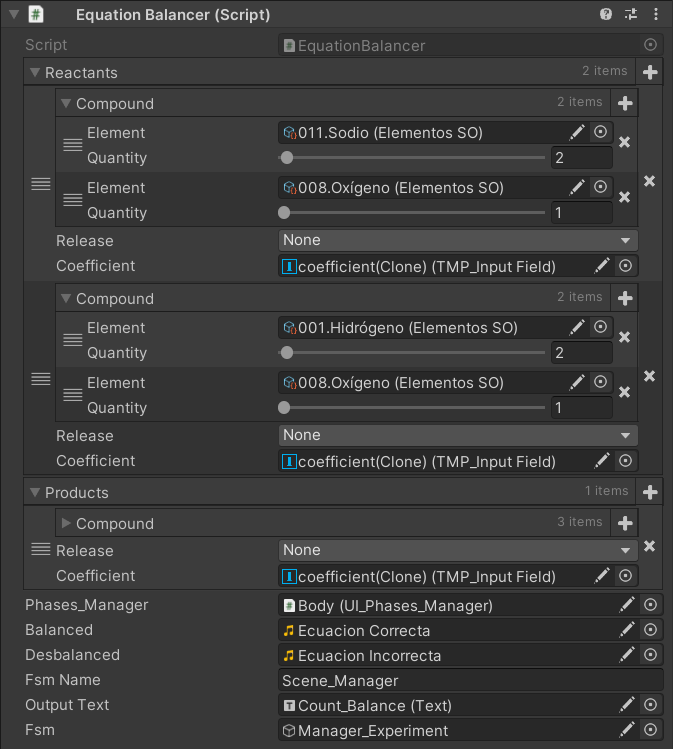
\includegraphics[width=0.45\textwidth, height = 6.75cm]{img/Equation_Balancer.png}
    \caption{Componente Equation Balancer en UNITY}
    \label{fig:Componente Equation Balancer en UNITY}
\end{figure}

Sus principales funciones incluyen:
\begin{itemize}
    \item Presentar ecuaciones químicas predefinidas al usuario en la interfaz.
    \item Evaluar los coeficientes ingresados para cada elemento químico, verificando que el balance sea correcto.
    \item Proporcionar retroalimentación inmediata, señalando errores y ofreciendo sugerencias para corregirlos.
\end{itemize}
\begin{figure}[thbp]
    \centering
    
\includegraphics[width=0.45\textwidth, height = 1.5cm]{img/Fórmula (2).png}
    \caption{Interfaz Balanceo de Ecuaciones}
    \label{fig:Interfaz Balanceo de Ecuaciones}
\end{figure}

\subsubsection{Periodic\_Table\_Manager}

Gestiona la tabla periódica interactiva, un elemento clave del simulador que permite la selección y el manejo de elementos químicos. 
\begin{figure}[thbp]
    \centering
    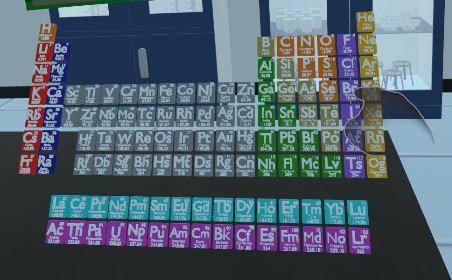
\includegraphics[width=0.45\textwidth, height = 5cm]{img/GUI/Tabla_Periodica.png}
    \caption{Tabla Periódica Interactiva}
    \label{fig:Tabla Periódica Interactiva}
\end{figure}
\\
Este módulo:
\begin{itemize}
    \item Instancia los modelos tridimensionales de los elementos seleccionados en el entorno de experimentación.
    \item Actualiza las interfaces gráficas (GUI) con información relevante sobre los elementos químicos.
    \item Se comunica con el \textbf{Manager\_experiment} para informar sobre las acciones realizadas por el usuario.
\end{itemize}
\begin{figure}[thbp]
    \centering
    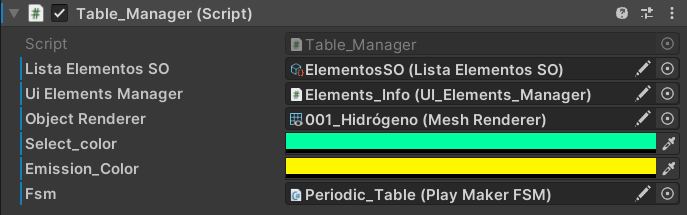
\includegraphics[width=0.45\textwidth, height = 2.75cm]{img/Table_Manager.png}
    \caption{Componente Table Manager en UNITY}
    \label{fig:Componente Table Manager en UNITYs}
\end{figure}
Es esencial durante las fases de selección y creación, proporcionando una herramienta visual y educativa que enriquece la experiencia del usuario.

\subsubsection{Compound\_Builder}

El módulo administra la creación, validación y representación de compuestos químicos. Actúa como intermediario entre la selección de elementos y el uso de instrumental, asegurando que los compuestos creados sean químicamente correctos\cite{Fernando2021}. 
\begin{figure}[thbp]
    \centering
    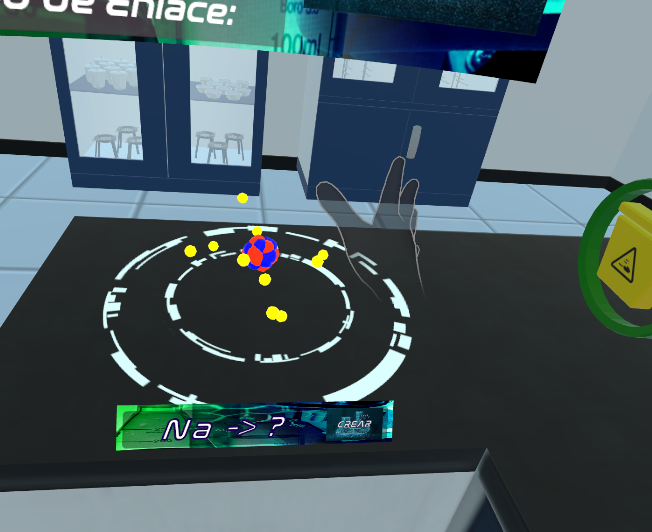
\includegraphics[width=0.45\textwidth, height = 5cm]{img/Zona_Creación (2).png}
    \caption{Zona de Creación de Compuestos}
    \label{fig:Zona de Creación de Compuestos}
\end{figure}

Entre sus funciones se incluyen:
\begin{itemize}
    \item Validación de combinaciones químicas según las reglas establecidas.
    \item Instanciación de modelos tridimensionales que representan los compuestos creados.
    \item Actualización de las interfaces gráficas con información detallada sobre los compuestos.
\end{itemize}
\begin{figure}[thbp]
    \centering
    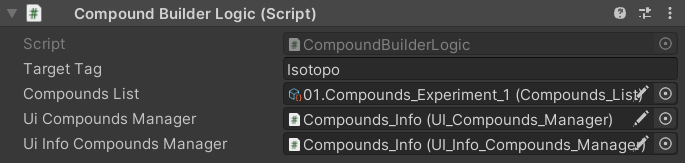
\includegraphics[width=0.45\textwidth, height = 2.75cm]{img/Compound_Builder.png}
    \caption{Componente Compound Builder en UNITY}
    \label{fig:Componente Compound Builder en UNITYs}
\end{figure}

\subsubsection{Instrumental}

El \textbf{instrumental} incluye todos los modelos tridimensionales de los equipos de laboratorio, como matraces, tubos de ensayo y mecheros. Cada componente está diseñado para replicar su funcionalidad en el entorno virtual\cite{alfa_nauta}\cite{Cinetica_Quimica_Basica}. 
\begin{figure}[thbp]
    \centering
    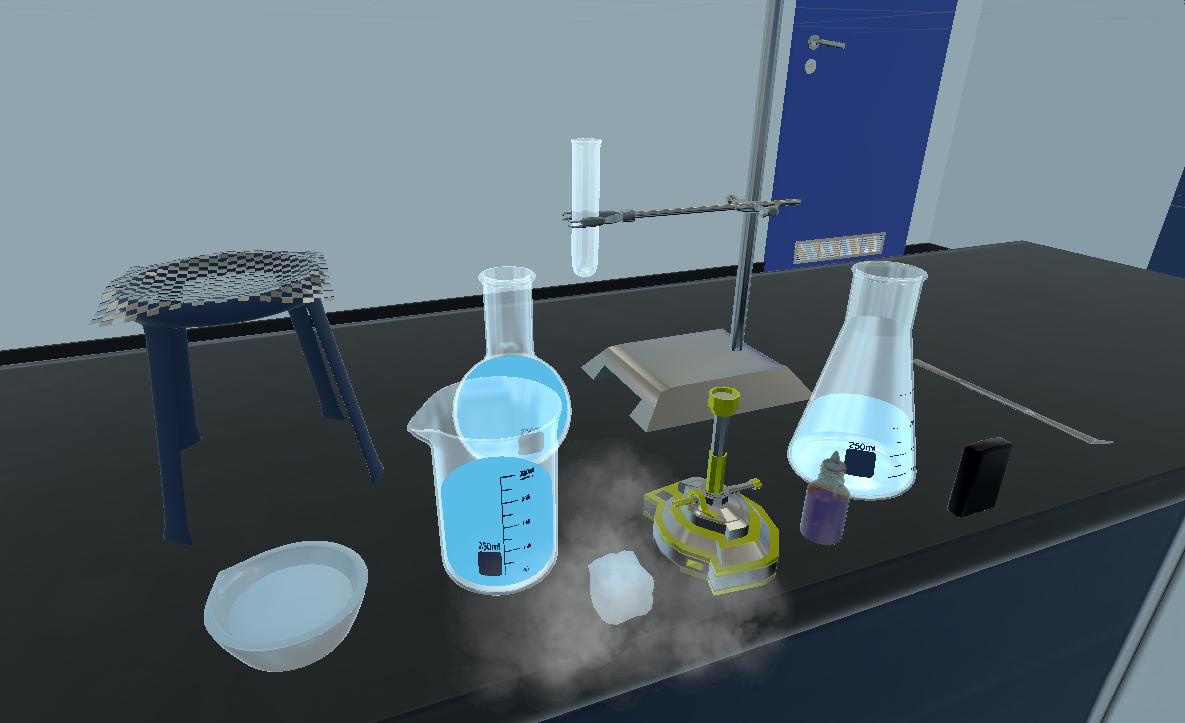
\includegraphics[width=0.45\textwidth, height = 5cm]{img/Instrumental.png}
    \caption{Instrumental de Laboratorio}
    \label{fig:Instrumental de Laboratorio}
\end{figure}

Este módulo integra:
\begin{itemize}
    \item \textbf{Simulación de Comportamientos:} Scripts que controlan acciones como mezcla, calentamiento y transferencia de líquidos.
    \item \textbf{Efectos Visuales y Sonoros:} Managers que enriquecen la experiencia inmersiva mediante efectos realistas.
    \item \textbf{Compatibilidad con \textit{Handtracking}:} Habilita la manipulación precisa de objetos mediante gestos naturales.
\end{itemize}

Dentro del módulo de instrumental, uno de los componentes más importantes es el \textbf{Liquid\_Manager}, diseñado específicamente para gestionar las acciones relacionadas con líquidos. Aunque no está presente en todos los instrumentales, este componente se encuentra integrado en elementos como matraces, probetas y recipientes de reacción, donde los líquidos desempeñan un papel fundamental.

Las principales responsabilidades del \textbf{Liquid\_Manager} incluyen:
\begin{itemize}
    \item \textbf{Gestión de Líquidos:} Controla la representación dinámica de los líquidos, incluyendo su nivel, color y reacciones físicas al interactuar con otros objetos o líquidos.
    \item \textbf{Simulación de Reacciones:} Integra efectos visuales y cambios químicos en los líquidos, como cambios de color, emisiones de vapor o formación de burbujas, en respuesta a las interacciones del usuario.
    \item \textbf{Interacciones Controladas:} Permite acciones como verter líquidos de un recipiente a otro, mezclar soluciones y observar los resultados de las reacciones simuladas.
\end{itemize}

\begin{figure}[thbp]
    \centering
    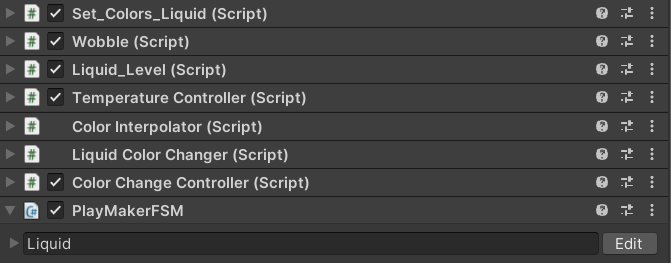
\includegraphics[width=0.45\textwidth, height = 3.5cm]{img/Componentes_de_Liquidos.png}
    \caption{Componentes de Líquidos}
    \label{fig:Componentes de Líquidos}
\end{figure}

El \textbf{Liquid\_Manager} asegura que los líquidos no solo sean representados visualmente, sino que también interactúen de manera coherente con el entorno y las herramientas del laboratorio. Esto permite al usuario experimentar con reacciones químicas y manipulaciones de líquidos en un entorno seguro, sin comprometer la precisión educativa. Su implementación se adapta a las necesidades de cada experimento, asegurando una experiencia inmersiva y funcional.

\begin{figure}[thbp]
    \centering
    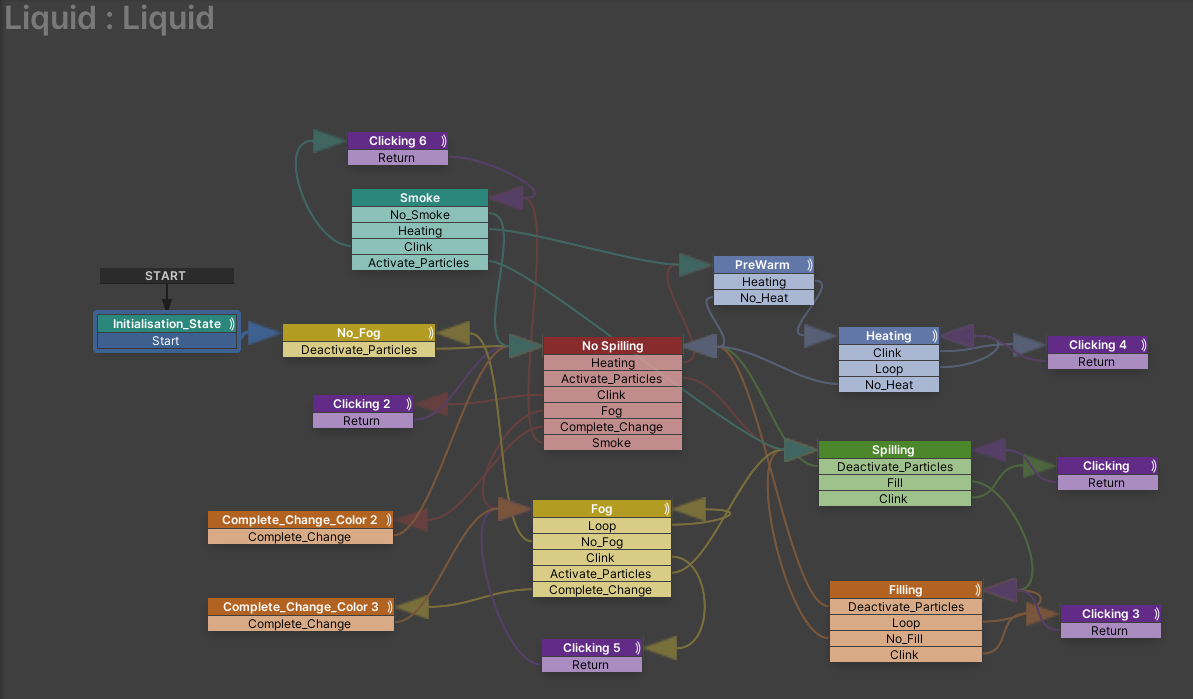
\includegraphics[width=0.45\textwidth, height = 5cm]{img/Liquids.png}
    \caption{Comportamiento de Líquidos}
    \label{fig:Comportamiento de Líquidos}
\end{figure}

\subsection{Limitaciones del Sistema}

El diseño del simulador presenta las siguientes limitaciones:
\begin{itemize}
    \item \textbf{Ámbito Exclusivo en Química Inorgánica:} No incluye experimentos de otras áreas de la química, como la orgánica o la bioquímica.
    \item \textbf{Experimentación Guiada:} Los experimentos disponibles son predefinidos y no permiten personalización.
    \item \textbf{Representación Simplificada:} Algunas propiedades químicas y reacciones se idealizan para facilitar la comprensión educativa.
    \item \textbf{Compatibilidad Limitada:} El simulador es compatible únicamente con dispositivos Oculus Meta Quest 2 y Meta Quest Pro.
\end{itemize}

\section{Resultados}

Se desarrolló un simulador de laboratorio de química inorgánica en realidad virtual que integra módulos funcionales para gestionar experimentos, balancear ecuaciones químicas, manipular elementos químicos y simular reacciones.\\

El sistema incluye cuatro experimentos y un tutorial introductorio, organizados en fases: introducción, balanceo de ecuaciones, selección y creación de compuestos, experimentación y retroalimentación.\\

Se realizaron pruebas de usuario con estudiantes de nivel secundaria, quienes interactuaron con el simulador para evaluar la experiencia educativa y la claridad de las actividades propuestas. Las observaciones cualitativas obtenidas permitieron realizar ajustes en las interfaces y las dinámicas de los experimentos.\\

El proyecto contó con el apoyo de un profesor de química, quien guió la selección de experimentos, asegurando su validez teórica, así como la representación correcta de los fenómenos químicos en el simulador.\\

Adicionalmente, el simulador fue presentado a diversos públicos para demostrar sus capacidades y recopilar comentarios cualitativos, los cuales ayudaron a refinar algunos aspectos de la experiencia de usuario.

\section{Conclusiones}

El desarrollo del prototipo de simulador de laboratorio de química inorgánica en realidad virtual permitió abordar una necesidad educativa específica mediante una herramienta tecnológica innovadora. Aunque existen otros simuladores en el ámbito de la química, pocos ofrecen una experiencia inmersiva y altamente interactiva, y menos aún están diseñados específicamente para un contexto educativo mexicano.\\

El prototipo implementó cuatro experimentos y un tutorial, permitiendo la realización de prácticas químicas con una representación visual y física detallada de los procesos involucrados. Estos elementos no solo enriquecen la experiencia del usuario, sino que también facilitan la comprensión de los conceptos químicos fundamentales.\\

Una característica distintiva del simulador es su enfoque en experimentos comúnmente realizados en aulas de nivel secundaria, lo que permite a los usuarios interactuar con prácticas químicas en un entorno virtual seguro y controlado. Esta experiencia fomenta un aprendizaje visual e interactivo, complementando la enseñanza tradicional de manera efectiva.\\

El prototipo desarrollado constituye una base sólida para futuras iteraciones que podrían ampliar su alcance y funcionalidad, mejorando aún más la enseñanza de la química mediante tecnologías inmersivas.

\section{Reconocimientos}
Los Autores agradecen a la Escuela Superior de Cómputo del Instituto Politécnico Nacional por el apoyo recibido y las facilidades otorgadas para el desarrollo del presente trabajo terminal

\begin{thebibliography}{9}

\bibitem{Brito2015}
A. Brito, ``Nuevas coordenadas para la alfabetización: debates, tensiones y desafíos en el escenario de la cultura digital,'' UNESCO IIEP Buenos Aires. Oficina para América Latina y Organización de Estados Iberoamericanos para la Educación, la Ciencia y la Cultura, Buenos Aires, 2015. [Online]. Available: \url{https://unesdoc.unesco.org/ark:/48223/pf0000371034.locale=es}. [Accessed: Sep. 14, 2023].

\bibitem{TrejoQuintana2020}
J. Trejo-Quintana, ``La falta de acceso y aprovechamiento de los medios y las tecnologías: dos deudas de la educación en México,'' in \textit{Educación y pandemia. Una visión académica}, México, 2020, pp. 122–128. [Online]. Available: \url{https://www.iisue.unam.mx/nosotros/covid/educacion-y-pandemia}. [Accessed: Sep. 14, 2023].

\bibitem{Zapatero2011}
D. Zapatero Guillén, ``La realidad virtual como recurso y herramienta útil para la docencia y la investigación,'' \textit{TEyET}, no. 6, pp. 17–23, Dec. 2011.

\bibitem{Zamorano2018}
T. Zamorano Escalona, Y. García Cartagena, and D. Reyes González, ``Educación para el sujeto del siglo XXI: principales características del enfoque STEAM desde la mirada educacional,'' \textit{Contextos: Estudios de Humanidades y Ciencias Sociales}, no. 41, Sep. 2018. [Online]. Available: \url{http://revistas.umce.cl/index.php/contextos/article/view/1386}. [Accessed: Sep. 17, 2023].

\bibitem{Estequiometria}
L. Gómez Chávez, “Stoichiometry,” \textit{PREPA3}, vol. 10, no. 19, pp. 58–59, Jan. 2023.

\bibitem{Fernando2021}
F. García Mata, “Leyes Ponderales,” \textit{Química General I}. Facultad de Química, UNAM, Departamento de Química Inorgánica y Nuclear, 2021. [Online]. Available: \url{https://drive.google.com/file/d/1knpRauxNInB-RMNJuajqGzBiA4q_qQcb/view}.

\bibitem{alfa_nauta}
J. L. Hernández, A. Violant, M. I. Binimelis, and J. L. Gutiérrez, “Química,” in \textit{alfa nauta - Programa Educativo Temático}. Ediciones Nauta C., S.A., Apr. 1997, pp. 171–289. ISBN: 84-89140-51-0.

\bibitem{Cinetica_Quimica_Basica}
H. E. Avery, \textit{Basic Reaction Kinetics and Mechanisms}. The Macmillan Press Ltd, 1974. ISBN: 978-0-333-15381-9. DOI: 10.1007/978-1-349-15520-0.
\end{thebibliography}


\end{document}
